\section{Appendix}
\frame{\frametitle{Agenda}\tableofcontents[currentsection]}
\subsection{Bottom-up -- Inverse Resolution}
\begin{frame}
	\frametitle{Bottom-up -- Inverse resolution [Muggleton '88]}
	Plotkins \textbf{LGG} Ansatz stark beschränkt

	Alternative Idee: \textbf{Inverse resolution}

	\begin{align*}
		B \wedge H &\vDash E \Leftrightarrow\\
		B \wedge \neg E &\vDash \neg H
	\end{align*}

	\vspace{5pt}

	Suchen einer \textit{Bridgefunktion} $F$:
	\vspace{5pt}
	\begin{align*}
		B \wedge \neg E     &\vDash F\\
		F                   &\vDash \neg H\\
		\Rightarrow \neg F  &\Dashv H\\
		\Rightarrow \neg F  &\succeq H\\
	\end{align*}
\end{frame}

\begin{frame}
	\frametitle{Bottom-up -- Inverse Resolution}
	Generelle Idee: Laufe den Herleitungsbaum rückwärts

	\begin{block}{Herleitungsbaum Aussagenlogik}
		Sei Theorie $\mathcal{T}=\{ u \leftarrow v; v \leftarrow w, w\}$ gegeben.
		Herleitung von $u$:
		\begin{figure}[H]
			\begin{center}
				\begin{tikzpicture}[scale=0.6]
					\node (A) at (0.3, 0) {$u$};
					\node (B) at (-3.6,2.15) {$u \leftarrow v$};
					\node (C) at (-2,4) {$v \leftarrow w$};
					\node (D) at (2,4) {$w$};
					\node (E) at (1.3, 2.2) {$v$};

					\path [->] (B) edge node[above] {} (A);
					\path [->] (C) edge node[above] {} (E);
					\path [->] (D) edge node[above] {} (E);
					\path [->] (E) edge node[above] {} (A);
				\end{tikzpicture}
			\end{center}
		\end{figure}
	\end{block}
\end{frame}

\begin{frame}
	\frametitle{Bottom-up -- Inverse Resolution}
	Herleitungen in \textit{First order logic} benötigt zusätzlich Substitutionen:

	\begin{itemize}
		\item $\mathcal{H} = \{c\} = \{daugther(X,Y) \leftarrow female(X), parent(Y,X)\}$
		\item $\mathcal{B} = \{b_1, b_2\}$ mit $b_1 = female(mary)$ und
			$b_2 = parent(ann, mary)$
		\item $\mathcal{T} = \mathcal{B} \cup \mathcal{H}$
		\begin{figure}[H]
			\begin{center}
				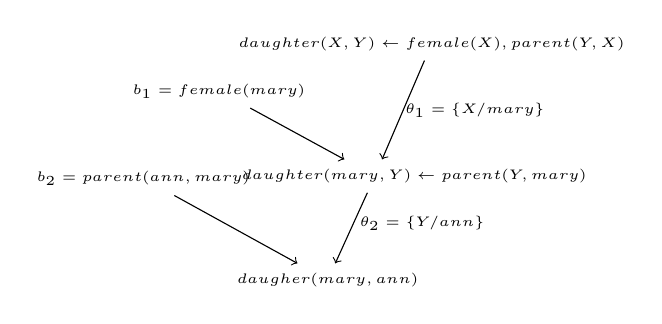
\begin{tikzpicture}[scale=0.6]
					\node (A) at (0.3, 0) {\tiny{$daugher(mary,ann)$}};
					\node (B) at (-3.6,2.15) {\tiny{$b_2 = parent(ann,mary)$}};
					\node (C) at (-2,4) {\tiny{$b_1 = female(mary)$}};
					\node (D) at (2.5,5) {\tiny{$daughter(X,Y) \leftarrow female(X), parent(Y,X)$}};
					\node (E) at (1.3, 2.2) {\hspace{1cm}\tiny{$daughter(mary, Y) \leftarrow parent(Y,mary)$}};
					\node (S1) at (2.3, 1.2) {\tiny{$\theta_2 = \{Y/ann\}$}};
					\node (S1) at (3, 3.6) {\hspace{0.5cm}\tiny{$\theta_1 = \{X/mary\}$}};


					\path [->] (B) edge node[above] {} (A);
					\path [->] (C) edge node[above] {} (E);
					\path [->] (D) edge node[above] {} (E);
					\path [->] (E) edge node[above] {} (A);
				\end{tikzpicture}
			\end{center}
		\end{figure}
	\end{itemize}
\end{frame}

\begin{frame}
	\frametitle{Bottom-up -- Inverse Resolution}
		\textbf{Inverse Substitution}: Umkehrung der Substitution:
		\begin{bsp}
			\begin{align*}
				c &= daughter(X, Y) \leftarrow female(X), parent(Y,X)\\
				\text{ mit } \theta &= \{X/mary, Y/ann\}\\
			\end{align*}
		\end{bsp}

		\begin{figure}[H]
			\begin{center}
				\begin{tikzpicture}[scale=0.6]
					\node[text width=3cm] (A) at (0, 0) {\tiny{$c' = daughter(mary, ann) \leftarrow female(mary),
					parent(ann, mary)$}};
					\node[text width=3cm] (B) at (8, 0) {\tiny{$c = daughter(X, Y)\leftarrow female(X), parent(Y,X)$}};
				    \path[dashed,->] (A) edge [red, bend left=70]  node[above] {$c'\theta$} (B);
					\path[dashed,->] (B) edge [blue, bend left=50]  node[above] {$c\theta^{-1}$} (A);
				\end{tikzpicture}
			\end{center}
		\end{figure}
\end{frame}

\begin{frame}
	\frametitle{Bottom-up -- Inverse Resolution}
	Inverse resolution beginnt mit $\mathcal{H} = \{\} = \emptyset$

	\begin{itemize}
		\item $\mathcal{B} = \{b_1,b_2\}$ mit $b_1 = female(mary)$ und
			$b_2 = parent(ann, mary)$
		\item Positives Beispiel $e_1 = daughter(mary, ann)$
	\end{itemize}
\end{frame}

\begin{frame}
	\frametitle{Bottom-up -- Inverse Resolution}
	Algorithmus:
	\begin{itemize}
		\item [1.] Finde Klausel $c_1$, sodass $\{b_2\} \cup c_1 \vDash e_1$
		\item [2.] Finde Klausel $c$\hspace{4pt}, sodass $\{b_1\} \cup c\hspace{4pt} \vDash c_1$
	\end{itemize}
		\begin{figure}[H]
			\begin{center}
				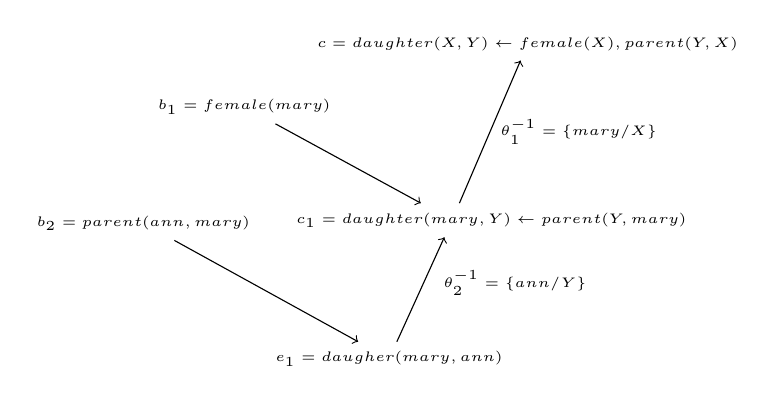
\begin{tikzpicture}[scale=0.8]
					\node (A) at (0.3, 0) {\tiny{$e_1 =daugher(mary,ann)$}};
					\node (B) at (-3.6,2.15) {\tiny{$b_2 = parent(ann,mary)$}};
					\node (C) at (-2,4) {\tiny{$b_1 = female(mary)$}};
					\node (D) at (2.5,5) {\tiny{$c = daughter(X,Y) \leftarrow female(X), parent(Y,X)$}};
					\node (E) at (1.3, 2.2) {\hspace{1cm}\tiny{$c_1 = daughter(mary, Y) \leftarrow parent(Y,mary)$}};
					\node (S1) at (2.3, 1.2) {\tiny{$\theta_2^{-1} = \{ann/Y\}$}};
					\node (S1) at (3, 3.6) {\hspace{0.5cm}\tiny{$\theta_1^{-1} = \{mary/X\}$}};


					\path [->] (B) edge node[above] {} (A);
					\path [->] (C) edge node[above] {} (E);
					\path [<-] (D) edge node[above] {} (E);
					\path [<-] (E) edge node[above] {} (A);
				\end{tikzpicture}
			\end{center}
		\end{figure}
\end{frame}

\begin{frame}
	\frametitle{Bottom-up -- Inverse Resolution}
	Zusammenfassung:
	Problem der \textit{Inverse resolution}:
	\begin{itemize}
		\item Nicht-deterministisch
		\item Hohe Komplexität (großer Suchraum)
	\end{itemize}
	$\Rightarrow$ Aktueller Gegenstand der Forschung
\end{frame}
\subsection{Saturierung}
\begin{frame}
	\frametitle{Appendix - Saturierung (Saturation)}
	\tikzstyle{vertex}=[circle,fill=black!25,minimum size=20pt,inner sep=0pt]
	\tikzstyle{vertex-red}=[circle,fill=red!24,minimum size=20pt,inner sep=0pt]
	\tikzstyle{edge} = [draw,thick,->]
	Background:
	\begin{align*}
		node(G,X)   \leftarrow red(G, X)\\
		node(G,X)   \leftarrow black(G,X)\\
		path(G,X,Y) \leftarrow arc(G,X,Y)\\
		path(G,X,Y) \leftarrow arc(G,X,Z), path(G,Z,Y), X \neq Z, Y \neq Z\\
	\end{align*}
	\begin{minipage}{0.5\textwidth}
	\begin{figure}
		\begin{tikzpicture}[scale=0.8, auto,swap]
			% Draw a 7,11 network
			% First we draw the vertices
			\node[vertex] (a) at (-1,2) {$a$};
			\node[vertex-red] (d) at (1,3) {$b$};
			\node[vertex] (b) at (2,1) {$c$};
			\node[vertex-red] (c) at (0,0) {$d$};
			% Connect vertices with edges and draw weights
			\foreach \source/ \dest in {a/d,d/c,c/d,d/b,b/c,c/a}
				\path[edge] (\source) edge [bend left=20] (\dest);
		\end{tikzpicture}
		\caption{Beispielgraph $g_1$}
	\end{figure}
	\end{minipage}
	\begin{minipage}{0.45\textwidth}
	Eigenschaften von $g_1$:
	\begin{gather*}
		black(g_1, a). \hspace{10pt} arc(g_1, a, b).\\
		red(g_1, b).   \hspace{10pt} arc(g_1, b, c). \\
		black(g_1, c). \hspace{10pt} arc(g_1, c, d). \\
		red(g_1, d).   \hspace{10pt} arc(g_1, d, a). \\
		arc(g_1, d, b).\hspace{10pt} arc(g_1, b, d).
	\end{gather*}
	\end{minipage}
\end{frame}

\begin{frame}
	\frametitle{Appendix - Saturierung (Saturation)}
	Saturierung von $g_1$ mit Hintergrundwissen, dass nur teilweise
	aus \textit{ground literals} besteht:
	\begin{align*}
		\begin{split}
		cyclic(g_1) \leftarrow &\;
		black(g_1, a) , arc(g_1, a, b), red(g_1, b)   , arc(g_1, b, c),\\
		&\;black(g_1, c) , arc(g_1, c, d), red(g_1, d) , arc(g_1, d, a),\\
		&\;arc(g_1, d, b), arc(g_1, b, d), path(g_1, a, c) ,path(g_1, a, c),\\
		&\;path(g_1, a, d) ,path(g_1, b, d) ,path(g_1, b, a) ,path(g_1, c, b),\\
		&\;path(g_1, c, a) ,path(g_1, d, c).
		\end{split}
	\end{align*}
\end{frame}
